\documentclass{ExcelAtFIT}

\usepackage{mathtools}
\usepackage{wrapfig}
\usepackage{listings}
\usepackage{parcolumns}
\usepackage{subcaption}
\usepackage{multirow}
\usepackage{pgf, tikz}
\usepackage{array}
\usepackage[normalem]{ulem}

\usetikzlibrary{arrows, automata, positioning}

\DeclareSymbolFont{newfont}{OML}{cmm}{m}{it}
\DeclareMathSymbol{\Varrho}{3}{newfont}{37}

\newcommand{\rulesep}{\unskip\ \vrule\ }

\newcommand{\tsf}[1]{{\color{cyan}TsF: #1}}

\newcolumntype{R}[1]{%
    >{\raggedleft\let\newline\\\arraybackslash\hspace{0pt}}m{#1}%
}

\renewcommand\vdots{\vbox{%
    \baselineskip3pt\lineskiplimit0pt\kern1pt%
    \hbox{.}\hbox{.}\hbox{.}\kern-1pt%
}}

\newtheorem{thm}{Theorem}
\newtheorem{lem}[thm]{Lemma}

\definecolor{darkgreen}{RGB}{53, 142, 5}
\newcommand{\bad}[1]{\textcolor{red}{\textbf{#1}}}
\newcommand{\good}[1]{\textcolor{darkgreen}{\textbf{#1}}}

\lstset{
    backgroundcolor=\color{white},
    basicstyle=\footnotesize\tt,
    language=C,
    showspaces=false,
    showtabs=false,
    tabsize=4,
    keepspaces=true,
    escapeinside={<@}{@>}
}

\DeclareMathAlphabet{\mathcal}{OMS}{cmsy}{m}{n}

%--------------------------------------------------------
%--------------------------------------------------------
%   REVIEW vs. FINAL VERSION
%--------------------------------------------------------

%   LEAVE this line commented out for the REVIEW VERSIONS
%   UNCOMMENT this line to get the FINAL VERSION
\ExcelFinalCopy

%--------------------------------------------------------
%--------------------------------------------------------
%   PDF CUSTOMIZATION
%--------------------------------------------------------

\hypersetup{
    pdftitle = {Scalable Static Analysis Using Facebook Infer},
    pdfauthor = {Dominik Harmim, Vladimír Marcin, Ondřej Pavela},
    pdfkeywords = {
        Facebook Infer, Static Analysis, Abstract Interpretation,
        Atomicity Violation, Concurrent Programs, Performance,
        Worst-Case Cost, Deadlock
    }
}

%--------------------------------------------------------
%--------------------------------------------------------
%   ARTICLE INFORMATION
%--------------------------------------------------------

\ExcelYear{2019}

\PaperTitle{Scalable Static Analysis Using Facebook Infer}

\Authors{Dominik Harmim*, Vladimír Marcin**, Ondřej Pavela***}
\affiliation{
    \{%
    *\href{mailto:xharmi00@stud.fit.vutbr.cz}{xharmi00},
    **\href{mailto:xmarci10@stud.fit.vutbr.cz}{xmarci10},
    ***\href{mailto:xpavel34@stud.fit.vutbr.cz}{xpavel34}%
    \}@stud.fit.vutbr.cz,
    \emph{%
        Faculty of Information Technology, Brno University
        of Technology%
    }
}

\Keywords{
    Facebook Infer ---
    Static Analysis ---
    Abstract Interpretation ---
    Atomicity Violation ---
    Concurrent Programs ---
    Performance ---
    Worst-Case Cost ---
    Deadlock
}

\Supplementary{
    \href{https://bitbucket.org/paveon/infer-performance/src/master}{
        Looper Repository***
    }
    --- \href{
        https://pajda.fit.vutbr.cz/xmarci10/fbinfer_concurrency/%
        tree/master
    }{
        L2D2 Repository**
    }
    --- \href{https://github.com/harmim/infer/tree/atomicity}{
        Atomer Repository*
    }
}

%--------------------------------------------------------
%--------------------------------------------------------
%   ABSTRACT and TEASER
%--------------------------------------------------------

\Abstract{
    \emph{Static analysis} has nowadays become
    one of the most popular ways of catching bugs
    early in the modern software. However, reasonably
    precise static analyses do still often have
    problems with scaling to larger codebases.
    And efficient static analysers, such
    as Coverity or Code Sonar, are often proprietary
    and difficult to openly evaluate
    or extend. \emph{Facebook Infer} offers a~static
    analysis framework that is open source, extendable,
    and promoting efficient modular
    and incremental analysis. In this work, we propose
    three \emph{inter-procedural} analysers extending the
    capabilities of Facebook Infer:
    \emph{Looper} (a~resource bounds analyser),
    \emph{L2D2} (a~low-level deadlock detector), and
    \emph{Atomer} (an atomicity violation analyser).
    We evaluated our analysers on both smaller
    hand-crafted examples as well as publicly available
    benchmarks derived from real-life low-level programs
    and obtained encouraging results. In particular,
    L2D2 attained 100\,\% detection rate and
    11\,\% false positive rate on an extensive benchmark
    of hundreds of functions and millions of lines of code.
}

% \Teaser{\TeaserImage{...}}

%--------------------------------------------------------
%--------------------------------------------------------
%--------------------------------------------------------
%--------------------------------------------------------
\begin{document}

\startdocument

%--------------------------------------------------------
%--------------------------------------------------------
%   ARTICLE CONTENTS
%--------------------------------------------------------

%--------------------------------------------------------
%--------------------------------------------------------
%--------------------------------------------------------
%--------------------------------------------------------
\section{Introduction}
Bugs are an inherent part of software ever since
the inception of the programming discipline.
They tend to hide in unexpected places, and when
they are triggered, they can cause significant
damage. In order to catch bugs early in the
development process, extensive automated testing
and dynamic analysis tools such as profilers are
often used. But while these solutions are sufficient
in many cases, they can sometimes still miss too
many errors. An alternative solution is a~\emph{static
analysis}, which has its own shortcomings as well.
Like, for example, a~high rate of \emph{false positives}
and, in particular, quite a~big problem with
\emph{scalability}.

Recently, Facebook has proposed its own solution
for efficient bug finding and program verification
called \emph{Facebook Infer}\,---\,a~highly
\emph{scalable} \emph{compositional} and
\emph{incremental} framework for creating
\emph{inter-procedural} analyses. Facebook Infer is still
under development, but it is in everyday use in
Facebook (and several other companies, such as
Spotify, Uber, Mozilla, and others) and it already
provides many checkers for various kinds of bugs,
e.g., for verification of buffer overflow, thread
safety, or resource leakage. However, equally
importantly, it provides a~suitable framework
for creating new analyses quickly.

However, the current version of Infer still misses
better support, e.g., for \emph{concurrency} or
\emph{performance-based} bugs. While it provides a~fairly
advanced \emph{data race} and \emph{deadlock} analysers,
they are limited to Java programs only and fail for
C~programs, which require more thorough manipulation with
locks. Moreover, the only performance-based analyser aims
to \emph{worst-case execution time} analysis only,
which does not provide a~wise understanding of
the programs performance.
% And while resource bounds analysis and concurrency
% checkers are not usable for all of the programs,
% they still can enhance both
% development process and user experience.

In particular, we propose to extend Facebook Infer
with three analysers: \emph{Looper}, a~resource
bounds analyser; \emph{L2D2}, a~lightweight
deadlock checker; and \emph{Atomer}, an atomicity
violation checker working on the level of sequence of
function calls. In experimental evaluation, we show
encouraging results, when even our immature
implementation could detect concurrency
property violations and infer precise bounds for
selected benchmarks, including rather large
benchmarks based on real-life code. The development
of these checkers has been discussed several times
with the developers of Facebook Infer, and it is an integral
part of the H2020 ECSEL project Aquas.

%--------------------------------------------------------
%--------------------------------------------------------
%--------------------------------------------------------
%--------------------------------------------------------
\section{Facebook Infer}
\label{sec:infer}

\emph{Facebook Infer} is an open-source static
analysis framework, implemented in OCaml, which is able to discover
various types of bugs of the given program, in
a~\emph{scalable} manner.
% Infer was originally
% a~standalone analyser focused on sound verification
% of absence of memory safety violations.
%which has made
%its breakthrough thanks to an influential
%paper~\cite{infer-biabduction}.
It is a~general \emph{abstract
interpretation}~\cite{CousotCousot77-1} framework
focused primarily on finding bugs rather than
formal verification that can be used to quickly
develop new kinds of \emph{compositional} and
\emph{incremental} analyses based on the notion
of function \emph{summaries}. In theory, a~summary
is a~representation of function's preconditions and
postconditions or effects. In practice,
it is a~custom data structure that allows
users to store arbitrary information resulting
from function's analysis. Infer does (usually) not
compute the summaries during a~run of the analysis
along the \emph{Control Flow Graph} (CFG) as is
done in classical analysers based on the ideas
from~\cite{Reps:1995:PID:199448.199462} and~\cite{Sharir:1981:CallStrings}.
Instead, it analyses a~program
\emph{function-by-function along the call tree}, starting
from its leafs. Hence, a~summary of a~function is
typically analysed without knowing its call context.
% This helps scalability (since summaries computed in
% different contexts are not distinguished), but it
% may easily lead to a~loss of precision.
The summary of the function is
then used at all of its call sites. Furthermore,
thanks to its incrementality, Infer can analyse
individual code changes instead of the whole project,
which is more suitable for large and quickly changing
codebases where the conventional batch analysis is
unfeasible. Intuitively, the incrementality is based
on re-using summaries of functions for which there is
no change in them nor in the functions (transitively)
called from them.

%The architecture of the Infer's abstract
%interpretation framework (Infer.AI) can be divided into
%three main component
%s as depicted in Figure~\ref{fig:inf-architecture}
%: a~frontend, an analysis scheduler, and a~collective set of
%analysis plugins.
% \begin{figure}[ht]
%   \centering
%   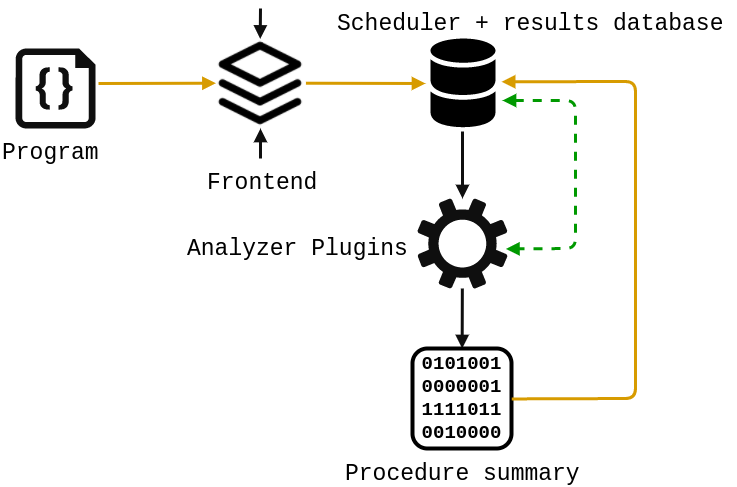
\includegraphics[scale=0.25]{images/infer/arch.png}
%   \caption{Infer's architecture components}
%   \label{fig:inf-architecture}
% \end{figure}

%The first component, the front-end, compiles input programs
%into the Smallfoot Intermediate
%Language (SIL) in a~form of the CFG.
%Each analysed procedure has its own
%CFG representation.
%The frontend supports multiple languages, so
%one can write (to some degree) language-independent analyses.

%The second component, the abstract interpreter or
%\textit{command interpreter},
% \begin{figure}[ht]
%   \centering
%   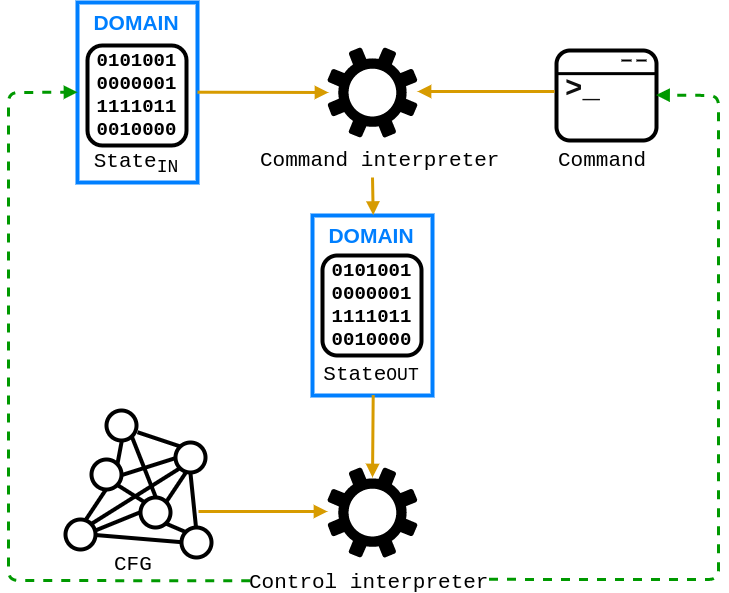
\includegraphics[scale=0.25]{images/infer/analysis.png}
%   \caption{The interpretation process in Infer}
%   \label{fig:infer-interpreter}
% \end{figure}
%subsequently interprets SIL
%instructions over input abstract states and produces new
%output states which are further scheduled for interpretation
%based on the CFG.
%Its simplified workflow is described in
%Figure~\ref{fig:infer-interpreter}.

Infer uses a~scheduler which determines the order of
analysis of individual functions based on a~\textit{call graph}.
It also checks if it is possible to analyse some functions
concurrently, which allows Infer to run in a~heavily
parallelized manner. In more detail, a~call
\begin{wrapfigure}{r}{0.23\textwidth}
    \centering
    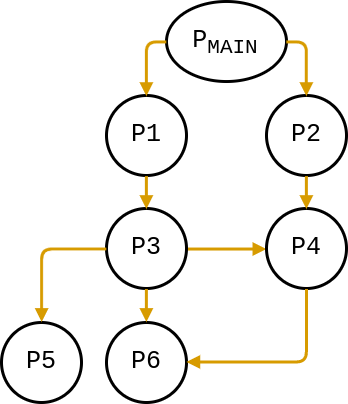
\includegraphics[width=0.23\textwidth]{images/infer/callgraph.png}
    \caption{A call graph}
    \label{fig:infer-callgraph}
\end{wrapfigure}
graph is a~\emph{directed graph}
describing call dependencies
between functions. An example of a~call graph is shown in
Figure~\ref{fig:infer-callgraph}. Using this figure, we can illustrate
the order of analysis in Infer and its incrementality.
The underlying analyser starts with the leaf functions $\mathtt{P5}$
and $\mathtt{P6}$
and then proceeds
towards the root $\mathtt{P_{MAIN}}$ while respecting
the dependencies represented by the edges.
% This order
% ensures that we will always have a~summary already
% available when we have to abstractly interpret
% a~nested function call during our analysis.
Each subsequent code change then triggers
a~re-analysis of the directly affected functions only
as well as a~re-analysis of all the functions up the call chain.
For example, if we modify the function $\mathtt{P3}$, Infer
will re-analyse only $\mathtt{P3}$,
$\mathtt{P1}$, and $\mathtt{P_{MAIN}}$.

Infer supports analysis of programs written in multiple
languages including C, C++, Objective-C, and Java and provides
a~wide range of analyses, each focusing on different types of bugs,
such as \textit{Inferbo} (buffer overruns),
\textit{RacerD}~\cite{racerd} (data races),
or \textit{Starvation} (concurrency starvation and
selected types of deadlocks).

%--------------------------------------------------------
%--------------------------------------------------------
%--------------------------------------------------------
%--------------------------------------------------------
\section{Worst-Case Cost Analyser}
\label{sec:worst-case-analyser}

Recently, performance issues have become
considerably more widespread in code, leading
to a~poor user experience. Facebook Infer
currently provides the \emph{cost}
checker~\cite{cost-checker} only, which implements
a~\emph{worst-case execution time} analysis
(\emph{WCET}). However, this analysis provides
a~numerical bound on the time required for the
execution of a~program only, which can be hard
to interpret, and, above all, it is quite
imprecise for more complex algorithms, e.g.,
requiring amortized reasoning.
Loopus~\cite{loopus-tool} is a~powerful resource
bounds analyser, which, to the best of our
knowledge, is the only one that can handle
\emph{amortized complexity analysis} for
a~broad range of programs. However, it is
limited to intra-procedural analysis only,
and the tool itself without an incremental
framework is not suitable for large and quickly
changing codebases. Hence, we implemented
\textit{Looper} -- analyser that recasts the
powerful analysis of Loopus within Infer which
enables the possibility for a~more efficient
resource bounds analysis.

Bounds inferred by Loopus refer to the number
of possible \textit{back jumps} to loop headers, which
is an useful metric related to
\textit{asymptotic time complexity} as it corresponds
to the possible number of executions of instructions
inside a~loop. The main algorithm relies on
an~abstract program model called
a~\textit{difference constraint program} (DCP), an example
of which can be seen in Figure~\ref{fig:foo_dcp}.
\vspace{-1mm}
\begin{lstlisting}[
caption=A snippet requiring amortized complexity
analysis. The DCP abstraction is shown in
Figure~\ref{fig:foo_dcp}. `*' denotes non-determinism.
Total cost: $3n$,
label={lst:foo}, mathescape=true]
void foo(int n):
    int i = n, j = 0, z = 0;
<@\textcolor{red}{$l_1:$}@>  while (i > 0):
        i--; j++;
<@\textcolor{red}{$l_2:$}@>      while (j > 0 && *) j--; z++;
    int x = z;
<@\textcolor{red}{$l_3:$}@>  while (x > 0) x--;
\end{lstlisting}

\begin{figure*}[ht]
\centering
\begin{subfigure}{.5\textwidth}
\centering
\bgroup
\def\arraystretch{1.15}
 \begin{tabular}{r|l}
 Call & Evaluation and Simplification\\ [0.25ex]
 \hline
 \multirow{3}{*}{
 $T\mathcal{B}(\tau_5)$} &
 $\rightarrow \mathtt{Incr}([x]) +
 $
 \\
 & $\quad T\mathcal{B}(\tau_4) \times
 \max(V\mathcal{B}([z]) + 0, 0)$\\
 &$\rightarrow 0 + 1 \times \max([n] + 0, 0) = [n]$\\
 \hline
 $V\mathcal{B}([z])$ & $\rightarrow
 \mathtt{Incr}([z]) + \max(V\mathcal{B}(0) + 0) = [n]$\\
 \hline
 $\mathtt{Incr}([z])$ & $\rightarrow T\mathcal{B}(\tau_2) \times 1
 = [n]$ \\
 \hline
 \multirow{2}{*}{$T\mathcal{B}(\tau_2)$} &
 $\rightarrow \mathtt{Incr}([j]) + T\mathcal{B}(\tau_0) \times 0$\\
 & $\rightarrow [n] + 1 \times 0 = [n]$ \\
 \hline
 $\mathtt{Incr}([j])$ & $\rightarrow T\mathcal{B}(\tau_1) \times 1
 = [n]$\\
 \hline
 \multirow{2}{*}{$T\mathcal{B}(\tau_1)$} &
 $\rightarrow \mathtt{Incr}([i]) + T\mathcal{B}(\tau_0) \times
 \max([n] + 0, 0)$\\
 & $\rightarrow 0 + 1 \times [n] = [n]$ \\
 \hline
\end{tabular}
\egroup
\caption{A simplified computation of the bound for
$\tau_5$. $\mathtt{Incr}([x])$ and $\mathtt{Incr}([i])$
are $0$ as there are no transitions that increase
the value of $[x]$ or $[i]$. $T\mathcal{B}(\tau_0)$ and
$T\mathcal{B}(\tau_4)$ are $1$ as they are not part of
any loop.}
\label{tbl:bound_computation}
\end{subfigure}%
\begin{subfigure}{.5\textwidth}
\centering
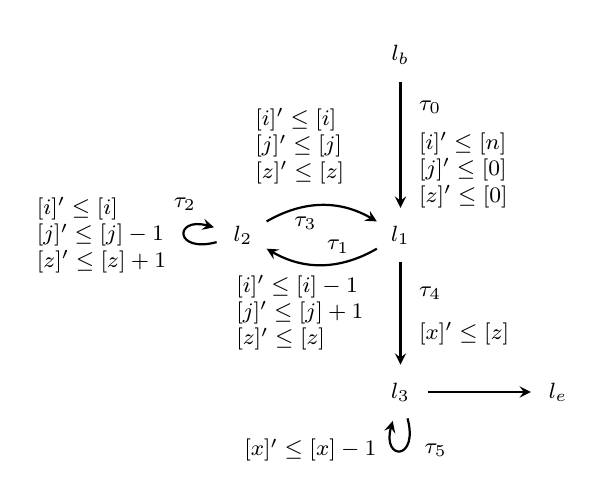
\begin{tikzpicture}[
    > = stealth, % arrow head style
    shorten > = 0pt,
    auto,
    node distance = 2cm, % distance between nodes
    thick, % line style
    font=\footnotesize
]

\tikzstyle{every state}=[
    draw = white,
    thick,
    fill = white,
    minimum size = 4mm,
]
\node[state] (lb) {$l_b$};
\node[state] (l1) [below=1.6cm of lb] {$l_1$};
\node[state] (l2) [left of=l1] {$l_2$};
\node[state] (l3) [below=1.3cm of l1] {$l_3$};
\node[state] (le) [right of=l3] {$l_e$};

\path[->] (lb) edge
node[right=3pt, pos=0.2]{$\tau_0$}
node[align=left, right=3pt, pos=0.7] {
$[i]' \leq [n]$\\
$[j]' \leq [0]$\\
$[z]' \leq [0]$} (l1);
\path[->] (l1) edge[bend left]
node[above, pos=0.35]{$\tau_1$}
node[align=left, below=1pt, pos=0.7] {
$[i]' \leq [i] - 1$\\
$[j]' \leq [j] + 1$\\
$[z]' \leq [z]$} (l2);

\path[->] (l2) edge[bend left]
node[pos=0.35, below]{$\tau_3$}
node[align=left, above=5pt, pos=0.3] {
$[i]' \leq [i]$\\
$[j]' \leq [j]$\\
$[z]' \leq [z]$} (l1);

\path[->] (l3) edge node {} (le);

\path[->] (l3) edge[loop below]
node[right=5pt]{$\tau_5$}
node[left=5pt] {$[x]' \leq [x] - 1$} (l3);

\path[->] (l1) edge
node[right=3pt, pos=0.3]{$\tau_4$}
node[align=left, right=3pt, pos=0.7] {
$[x]' \leq [z]$} (l3);

\path[->] (l2) edge[loop left]
node[align=left, left=3pt] {
$[i]' \leq [i]$\\
$[j]' \leq [j] - 1$\\
$[z]' \leq [z] + 1$}
node[above=5pt] {$\tau_2$} (l2);
\end{tikzpicture}
\caption{An abstraction obtained from Listing~\ref{lst:foo}.
Each transition is denoted by a~set of invariant
inequalities.}
\label{fig:foo_dcp}
\end{subfigure}
\caption{}
\label{fig:loopus_example}
\end{figure*}

Each transition $\tau$ of a~DCP has
a~\textit{local bound} $\tau_{v}$, i.e., a~variable
$v$ that \textit{locally} limits the number of
executions of the transition $\tau$. For example, the variable $j$ in
Figure~\ref{fig:foo_dcp} limits the number of consecutive
executions of the transition $\tau_2$.

The bound algorithm is based on the idea of
reasoning about \textit{how often} and
\textit{by how much} might the local bound of
a~transition $\tau$ increase, which affects
the number of executions of $\tau$. The computation
interleaves calls to two procedures:
\vspace{-2.5mm}
\begin{enumerate}
    \item $V\mathcal{B}$\,--\,computes
    a~\textit{variable bound} expression in terms of
    program parameters which bounds the value of the
    variable $v$.

    \item $T\mathcal{B}$\,--\,computes a~bound on the
    number of times that a~transition $\tau$ can be
    executed. Transitions that are not part of any
    loop have the transition bound $1$.
\vspace{-2.5mm}
\end{enumerate}
The $T\mathcal{B}$ procedure is defined in the following
way:
\setlength{\belowdisplayskip}{3pt}
\setlength{\abovedisplayskip}{3pt}
\begin{linenomath}
\begin{equation*}
T\mathcal{B}(\tau) =
\mathtt{Incr}(\tau_v) +
\mathtt{Resets}(\tau_v)
\end{equation*}
\end{linenomath}
The $\mathtt{Incr}(\tau_v)$ procedure
represents \textit{how often}
and \textit{by how much} might the local bound
$\tau_v$ increase:
\begin{linenomath}
\begin{equation*}
\mathtt{Incr}(\tau_v)=
\sum\limits_{(\mathtt{t, c})\in
\mathcal{I}(\tau_v)}
T\mathcal{B}(\mathtt{t})\times\mathtt{c}
\label{eq:incr_procedure}
\end{equation*}
\end{linenomath}
$\mathcal{I}(\tau_v)$ is the set of transitions
$\mathtt{t}$ that increase the value of $\tau_v$
by $\mathtt{c}$. $\mathtt{Resets}(\tau_v)$
represent the possible resets of the local bound
$\tau_v$ to some arbitrary values which also add
to the total amount by which $\tau_v$ and
consequently $T\mathcal{B}(\tau)$ might increase:
\begin{linenomath}
\begin{equation*}
\mathtt{Resets}(\tau_v)=
\sum\limits_{(\mathtt{t, a, c})\in
\mathcal{R}(\tau_v)}
T\mathcal{B}(\mathtt{t})\times
\mathrm{max}(V\mathcal{B}(\mathtt{a}) + \mathtt{c}, 0)
\label{eq:resets_procedure}
\end{equation*}
\end{linenomath}
Above, $\mathcal{R}(\tau_v)$ is the set of transitions
$\mathtt{t}$ that reset the value of the local bound
$\tau_v$ to $\mathtt{a} + \mathtt{c}$ where $\mathtt{a}$
is a~variable.

The remaining $V\mathcal{B}(\mathtt{v})$ procedure
is defined as:
\begin{linenomath}
\begin{equation*}
V\mathcal{B}(\mathtt{v}) =
\mathtt{Incr}(\mathtt{v}) +
\max\limits_{(\mathtt{t, a, c})\in
\mathcal{R}(\mathtt{v})}(
V\mathcal{B}(\mathtt{a}) + \mathtt{c})
\end{equation*}
\end{linenomath}
It picks the maximal value of all possible resets of
$\mathtt{v}$ as the initial value and increases it by
the value of $\mathtt{Incr(v)}$. Note that the
procedure returns $\mathtt{v}$ itself if it is
a~program parameter or a~numeric constant.

The complete bound algorithm is then
the mutual recursion of the procedures $T\mathcal{B}$
and $V\mathcal{B}$. The main reason why Loopus scales
so well with this approach is \textit{local} reasoning:
it does not rely on any global program  analysis and
is able to obtain complex invariants  such as
$x \leq \max(m1,m2) + 2n$. These invariants
are not expressible in common abstract domains such
as \textit{octagon} or \textit{polyhedra}, which
would lead to a~less precise result. This approach
is also \textit{demand-driven}
(Figure~\ref{tbl:bound_computation}), i.e. it only
performs necessary recursive calls and does not
compute all possible invariants. For a~full
\textit{flow} and \textit{path sensitive} algorithm
and its extension refer to~\cite{loopus-tool}.

Figure~\ref{tbl:bound_computation} presents an
example computation of the transition bound of
$\tau_5$ from the DCP in Figure~\ref{fig:foo_dcp},
which corresponds to Listing~\ref{lst:foo}. This code
demonstrates
the need for amortized complexity analysis as the
worst-case cost of the $l_2$ loop can indeed be
$n$. However, its amortized cost is $1$ as the
total number of iterations of $l_2$ (total cost) is also equal
to $n$ due to the local bound $j$, which is bounded by
$n$. Loopus is able to obtain the bound of $n$ instead
of $n^2$ for the inner loop $l_2$ unlike many other tools.
Another challenge is the computation of
the bound for the loop $l_3$. It is easy to infer $z$
as the bound, but the real challenge lies in expressing
the bound in terms of program parameters. Thus, the
real task is to obtain an invariant of the form
$z \leq \mathtt{expr}(n)$ where $\mathtt{expr}(n)$
denotes an expression over program parameters,
$n$ in this case. Loopus is able to obtain the
invariant $z \leq n$ simply with the $V\mathcal{B}$
procedure and to infer the bound $n$ for
the loop $l_3$.

The implementation of $T\mathcal{B}$ and
$V\mathcal{B}$ is quite straightforward in
a~functional paradigm (OCaml). We first convert
the native CFG used by Infer into a~DCP used
by Loopus' abstraction. In particular, we
leverage the AI framework and symbolically
execute the~program yielding a~transition system.
Further, we had to implement the abstraction
algorithm and an algorithm which computes local
bounds. We further extended the basic algorithm
with several extensions which improve its precision
such as a~reasoning based on so called
\textit{reset chains} or an algorithm that converts
the standard DCP into a~\textit{flow-sensitive} one
by variable renaming. For more details about these
extensions, refer to~\cite{loopus-tool}. The current
implementation is still limited to intra-procedural
analysis as the original Loopus. However, we already
have a~conceptual idea based on substitution of the
formal parameters in a~symbolic bound expression stored
in a~summary with the variable bounds of arguments at
a~callsite resulting in, albeit less precise, but
scalable solution. We should also be able to obtain
the symbolic return value through the $V\mathcal{B}$
procedure and then use it at a~call site in a~similar
way. We are aware that this reasoning is limited to
functions without pointer manipulation but it should
be a~step in the right direction.

Table~\ref{tbl:loopus_evaluation} presents experimental
results of our current implementation on selected
examples from the dissertation~\cite{loopus-tool}.
We compared the results of \textit{Looper}
(Loopus in Infer) with the \textit{Cost} analyser
mentioned in the introduction of this section.
For \textit{Cost} we have simplified the reported
bounds to the worst-case asymptotic complexity
instead of the cost.

\begin{table}[t]
\centering
\caption{An experimental evaluation of \textit{Looper}.
Benchmarks are publicly available\protect\footnotemark.}
\def\arraystretch{1}
 \begin{tabular}{|c|r||R{1.3cm}|R{1cm}||R{1.3cm}|R{1cm}|}
 \hline
 \multirow{2}{*}{} & \multirow{2}{*}{Bound} &
 \multicolumn{2}{|c||}{Inferred bound} &
 \multicolumn{2}{|c|}{Time [s]}\\
 \cline{3-6}
 & & \multicolumn{1}{|c|}{Looper} &
 \multicolumn{1}{|c||}{Cost} &
 \multicolumn{1}{|c|}{Looper} &
 \multicolumn{1}{|c|}{Cost}\\
 \hline
 \hline
 \#1 & $n$ & \bad{$2n$} & \bad{$n^2$} & 0.3 & 0.4\\
 \hline
 \#2 & $2n$ & \good{$2n$} & \bad{$5n$} & 0.5 & 0.4\\
 \hline
 \#3 & $4n$ & \bad{$5n$} & \bad{$\infty$} & 0.8 & 1.4\\
 \hline
 \#4 & *$n^2$ & \good{$n^2$} & \bad{$\infty$} & 0.6 & 0.9\\
 \hline
 \#5 & $2n$ & \good{$2n$} & \bad{$12n$} & 0.3 & 0.5\\
 \hline
 \#6 & *$n$ & \good{$n$} & \bad{$\infty$} & 0.6 & 0.7\\
 \hline
 \#7 & $2n$ & \good{$2n$} & \bad{$\infty$} & 0.4 & 1\\
 \hline
 \#8 & $2n$ & \good{$2n$} & \bad{$\infty$} & 0.7 & 1.8\\
 \hline
\end{tabular}
\label{tbl:loopus_evaluation}
\vspace{-5mm}
\end{table}
\footnotetext{\url{https://bit.ly/2uORslv}}

%--------------------------------------------------------
%--------------------------------------------------------
%--------------------------------------------------------
%--------------------------------------------------------
\section{Deadlock Analyser}
\label{sec:deadlock-analyser}

According to~\cite{dogru2011modern}, deadlock is perhaps the most common concurrency error that might occur in almost all parallel programming paradigms including both shared-memory and distributed memory. Detecting deadlocks during testing is very hard due to many possible interleavings among threads. Of course, one can use extrapolating dynamic analysers and/or techniques such as noise injection or systematic testing~\cite{conErrors} to increase chances of finding deadlocks, but such techniques decrease the scalability of the testing process and can still have problems discovering some errors. That is the reason why many static detectors were created, but most of them are quite heavy-weight and do not scale well. However, there are few that meet the scalability condition, like the \textit{starvation} analyser implemented in Facebook Infer. But, the problem of this analyser is that it uses a~heuristic based on using the class of the root of the \emph{access path}\footnote{Infer uses access paths for naming heap locations via the paths used to access them, e.g., \texttt{x.f.g} (\texttt{x} is the root).} of a~lock, and so it does not handle pure C~locks. Another, that is worth mentioning, is the RacerX analyser~\cite{racerx}, which is based on counting so-called \textit{locksets}, i.e., sets of locks currently held. RacerX uses interprocedural, flow-sensitive, and context-sensitive analysis. This means that each function needs to be reanalysed in a~new context, which reduces the scalability. Hence, we have decided to develop a~new context-insensitive analysis (only very loosely inspired by RacerX), which will be faster and more scalable. We have implemented this analysis in our \textit{Low-Level Deadlock Detector (L2D2)}, the principle of which will be illustrated by the example in Listing~\ref{deadlock_example} (a~full description of the algorithm with all its optimisations is beyond the scope of this paper).

L2D2 works in two phases. In the first phase, it computes a~summary for each function by looking for lock and unlock events present in the function. An example of a~lock and an unlock event is illustrated in Listing~\ref{deadlock_example} at lines 22 and 27. If a~call of a~user-defined function appears in the analysed code during the analysis, like at line 26 of our example, the analyser is provided with a~summary of the function if available. Otherwise, the function is analysed on demand (which effectively leads to analysing the code along the call tree, starting at its leaves, as usual in Facebook Infer). The summary is then applied to an abstract state at the call site. Hence, in our example, the summary of \texttt{foo} will be applied to the abstract state of \texttt{thread1}. More details on what the summaries look like and how they are computed will be given in Section~\ref{summ_computation}.
\begin{lstlisting}[float=tp, belowskip=-1.5 \baselineskip, caption= A~simple example capturing a~deadlock between two global locks in the C~language using the POSIX threads execution model,
label={deadlock_example}, mathescape=true]
16 void foo() {
17     pthread_mutex_lock(<@\textcolor{blue}{\&lock2}@>);
21 void *thread1($\dots$) {
22     pthread_mutex_lock(<@\textcolor{red}{\&lock1}@>);
     $\hspace{20pt}\vdots$
26     foo();
27     pthread_mutex_unlock(<@\textcolor{red}{\&lock1}@>);
29 void *thread2($\dots$) {
30     pthread_mutex_lock(<@\textcolor{blue}{\&lock2}@>);
     $\hspace{20pt}\vdots$
36     pthread_mutex_lock(<@\textcolor{red}{\&lock1}@>);
\end{lstlisting}
\begin{lstlisting}[float=bp, aboveskip=-1 \baselineskip, label={deadlock_example_summary}, caption=Summaries of the functions in Listing~\ref{deadlock_example}]
<@\textbf{foo()}@>
  PRECONDITION: { unlocked={lock2} }
  POSTCONDITION: { lockset={lock2} }
<@\textbf{thread1(\dots)}@>
  PRECONDITION: { unlocked={lock1, lock2} }
  POSTCONDITION: { lockset={lock2},
    dependencies={lock1->lock2} }
<@\textbf{thread2(\dots)}@>
  PRECONDITION: { unlocked={lock1, lock2} }
  POSTCONDITION: { lockset={lock1, lock2},
    dependencies={lock2->lock1} }
\end{lstlisting}

In the second phase, L2D2 looks through all the computed summaries of the analysed program and concentrates on so-called \textit{dependencies} that are part of the summaries. The dependencies record that some lock got locked at a~moment when another lock was still locked. L2D2 interprets the obtained set of dependencies as a~relation, computes its transitive closure, and reports a~deadlock if some lock depends on itself in the transitive closure.

%todo postpone this example after the summaries explanation
If we run L2D2 on our example, it will report a~possible deadlock due to the cyclic dependency between \texttt{lock1} and \texttt{lock2} that arises if thread 1 holds \texttt{lock1} and waits on \texttt{lock2} and thread 2 holds \texttt{lock2} and waits on \texttt{lock1}. This is caused by dependencies \texttt{lock1$\rightarrow$lock2} and \texttt{lock2$\rightarrow$lock1} in the summaries of \texttt{thread1} and \texttt{thread2}
(see Listing~\ref{deadlock_example_summary}).

\subsection{Computing Function Summaries}
\label{summ_computation}
We now describe the structure of the summaries used and the process of computing them. To detect potential deadlocks, we need to record information that will allow us to answer the following questions:
\begin{enumerate}[label={(\arabic*)}, topsep=0.4em]
    \item \label{q1} What is the state of the locks used in the analysed program at a~given point in the code?
    \item \label{q2} Could a~cyclic dependency on pending lock requests occur?
\end{enumerate}

To answer question~\ref{q1}, we compute sets \textit{lockset} and \textit{unlockset}, which contain the currently locked and the currently unlocked locks, respectively. These sets are a~part of the \textit{postconditions} of functions and record what locks are locked/unlocked upon returning from a~function, respectively. Further, we also compute sets \textit{locked} and \textit{unlocked} that serve as a~\textit{precondition} for a~given function and contain locks that should be locked/unlocked before calling this function.
When analysing a~function, the sets are manipulated as shown in Figure \ref{summary_rules}.

Each summary contains also a~set of \textit{dependencies} using which we can answer question $\ref{q2}$. Extraction of the dependencies is called upon every lock acquisition and iterates over every lock in the current lockset, emitting the ordering constraint produced by the current acquisition. For example, if \texttt{lock2} is in the current lockset and \texttt{lock1} has just been acquired, the dependency \texttt{lock2$\rightarrow$lock1} will be emitted, as we can see in Listing~\ref{deadlock_example} in the function \texttt{thread2}.
\begin{lstlisting}[mathescape=true, keywordstyle=\ttfamily, float=tp, belowskip=-1 \baselineskip, label={summary_rules}, caption=Rules for summary computation ]
<@\textbf{lockset:}@>
  lock(l) $\rightarrow$ lockset := lockset $\cup$ {l}
  unlock(l) $\rightarrow$ lockset := lockset - {l}
<@\textbf{unlockset:}@>
  lock(l) $\rightarrow$ unlockset := unlockset - {l}
  unlock(l) $\rightarrow$ unlockset := unlockset $\cup$ {l}
<@\textbf{locked:}@>
  if(lock(l) is the first operation in $f$)
    unlocked$_f$ := unlocked$_f$ $\cup$ {l}
<@\textbf{unlocked:}@>
  if(unlock(l) is the first operation in $f$)
    locked$_f$ := locked$_f$ $\cup$ {l}
\end{lstlisting}


% todo
The above described basic computation of the dependencies would, however, be very imprecise and lead to many false alarms. The imprecision is caused by invalid locksets. The main reasons for imprecision of the locksets are imprecision in dealing with conditionals (all outcomes are considered as possible), with function calls (missing context), and with lock aliasing (any aliasing is considered to be possible).



% todo maybe drop
% \subsection{Reporting Deadlocks}
% For deadlock detection, we use an algorithm that iterates through all the summaries and computes the transitive closure of all dependencies. It records the cyclic lock dependency and displays the results to the user for inspection. Each deadlock (between two locks) is normally reported twice, for each locking event that can be considered a~beginning of the cyclic locking dependency separately. So, in our example in Listing~\ref{deadlock_example}, we will report the deadlock for the first time in function \texttt{thread1} and for the second time in function \texttt{thread2}.

\subsection{Experimental Evaluation}
We performed experiments using a~benchmark of 1002 concurrent C~programs derived from the Debian GNU Linux distribution.The entire benchmark is available online at GitLab. These programs were originally used for an experimental evaluation of Daniel Kroening's static deadlock analyser~\cite{cprover} implemented in the CPROVER framework.

This benchmark set consists of 11.4 MLOC. Of all the programs, 994 are deadlock-free and 8 of them contain a~deadlock. Our experiments were run on a~CORE i7-7700HQ processor at 2.80\,GHz running Ubuntu 18.04 with 64-bit binaries. The CPROVER experiments were run on a~Xeon X5667 at 3\,GHz running Fedora 20 with 64-bit binaries. In case of CPROVER, the memory and the CPU time were restricted to 24\,GB and 1800 seconds per benchmark, respectively.

Both our analyser and CPROVER correctly report all 8 potential deadlocks in the benchmarks with known issues. A~comparison of results for deadlock-free programs can be seen in Table~\ref{tbl:DeadlockBanch}.

As one can see, L2D2 reported false alarms for 104 deadlock-free benchmarks which is by 10 less than CPROVER. A~much larger difference can be seen in cases where it was proved that there was no deadlock. The difference here is 518 examples in favor of our analyser. In case of L2D2, we have 80 compilation errors that were caused by syntax that Infer does not support. The biggest difference between our analyser and CPROVER is the runtime. While our analyser needed approximately 2 hours to perform the experiments, CPROVER needed about 300 hours.
\begin{table}[t]
\caption{Results for programs without a~deadlock (t/o\,---\,timed out, m/o\,---\,out of memory)}
\begin{tabular}{l|r|r|r|r|r}
        & \multicolumn{1}{l|}{\textbf{proved}} & \multicolumn{1}{l|}{alarms} & \multicolumn{1}{l|}{t/o} & \multicolumn{1}{l|}{m/o} & \multicolumn{1}{l}{errors} \\ \hline
CPROVER & \textbf{292}                        & 114                        & 453                     & 135                     & 0                          \\
L2D2    & \textbf{810}                        & 104                        & 0                       & 0                       & 80
\end{tabular}
\label{tbl:DeadlockBanch}
\vspace{-5mm}
\end{table}

There is still space for improving our analysis by reducing the number of alarms, which are mainly caused by false dependencies as mentioned in Subsection~\ref{summ_computation} ($4^{th}$ paragraph). Hence, to eliminate false positives, we need some techniques to eliminate false dependencies. In our implementation of L2D2, we use a~number of heuristics that try to reduce the imprecision. An example is that if a~locking error occurs (double lock acquisition), then L2D2 sets the current lockset to empty, and adds the currently acquired lock to the lockset (we can safely tell that this lock is locked), thereby eliminating any dependencies that could result from the locking error. More precise description of these heuristics is beyond the scope of the paper.

%--------------------------------------------------------
%--------------------------------------------------------
%--------------------------------------------------------
%--------------------------------------------------------
\section{Atomicity Violations Analyser}

In \emph{concurrent programs} there are often
\emph{atomicity requirements} for execution of specific
sequences of instructions. Violating these requirements
may cause many kinds of problems, such as an unexpected
behaviour, exceptions, segmentation faults, or other
failures. \emph{Atomicity violations} are usually not
verified by compilers, unlike syntactic or some sorts
of semantic rules. Atomicity requirements,
in most cases, are not even documented. It means
that typically only programmers must take care of
following these requirements. In general, it is very
difficult to avoid errors in \emph{atomicity-dependent
programs}, especially in large projects, and even harder
and time-consuming is finding and fixing these errors.

In this section we propose
an implementation of a~\emph{static analyser for
finding atomicity violations}. In particular,
we concentrate on an \emph{atomic execution
of sequences of function calls}, which is often
required, e.g., when using certain library calls.

\subsection{Contracts for Concurrency}
\label{sec:contracts}

The proposal of a~solution is based on the concept of
\emph{contracts for concurrency} described
in~\cite{atomicity-contracts}. These contracts
allow one to define \emph{sequences of functions} that are
required to be \emph{executed atomically}. The proposed
analyser itself (\textbf{Atomer}) is able to automatically
derive candidates for such contracts, and then to verify
whether the contracts are fulfilled.

In~\cite{atomicity-contracts},
a~\emph{basic contract} is formally defined as follows.
Let $ \Sigma_\mathbb{M} $~be a~set of all function names
of a~software module. A~\emph{contract} is
the set $ \mathbb{R} $~of \emph{clauses} where each
clause $ \Varrho\ \in \mathbb{R} $~is a~regular
expression over $ \Sigma_\mathbb{M} $.~A~\emph{contract
violation} occurs if any of the sequences represented by
the contract clauses is interleaved with an execution of
functions from $ \Sigma_\mathbb{M} $.

Consider an implementation of a~function that replaces
item \texttt{a}~in an array by item \texttt{b},
illustrated in Listing~\ref{list:contracts}. The contract
for this specific scenario contains
clause $ \Varrho_1 $,~which is defined as follows:
\\[0.4em]
\centerline{$
    (\Varrho_1)\ \text{\texttt{index\_of~set}}
$}
\\[0.4em]
Clause $ \Varrho_1 $~specifies that every execution
of \texttt{index\_of} followed by an execution of
\texttt{set} should be atomic. The index of an
item in an array is acquired, and then the index
is used to modify the array. Without atomicity,
a~concurrent modification of the array may change
a~position of the item. The acquired index may
then be invalid when \texttt{set} is executed.

\begin{lstlisting}[
    float=tp, belowskip=-1.6 \baselineskip,
    label={list:contracts},
    caption={An example of a~contract violation}
]
void replace(int *array, int a, int b):
    int i = index_of(array, a);
    if (i >= 0) set(array, i, b);
\end{lstlisting}

In~\cite{atomicity-contracts} there is described
a~proposal and an implementation of a~\emph{static
validation for finding atomicity violations},
which is based on \emph{grammars} and
\emph{parsing trees}. The authors
of~\cite{atomicity-contracts} implemented
the stand-alone prototype
tool\footnote{\url{https://github.com/trxsys/gluon}} for
analysing programs written in Java, which
led to some promising experimental results but the
\emph{scalability} of the tool was still limited. Moreover,
the tool from~\cite{atomicity-contracts} is no more
developed. That is why we decided to get inspired
by~\cite{atomicity-contracts} and reimplement the
analysis in \emph{Facebook Infer} redesigning it in
accordance with the principles of Infer, which
should make it more \emph{scalable}. In the end,
due to adapting the analysis for the context of Infer,
our implementation is significantly different
from~\cite{atomicity-contracts} as presented in
Sections~\ref{sec:atomicity-phase1} and \ref{sec:atomicity-phase2}.
Furthermore, unlike~\cite{atomicity-contracts},
the implementation aims at programs written in
C/C++ languages using \emph{POSIX Threads (Pthreads)}
locks for \emph{synchronisation of concurrent
threads}.

In Facebook Infer there is already implemented
an analysis called
\href{https://fbinfer.com/docs/checkers-bug-types.html\#LOCK_CONSISTENCY_VIOLATION}{Lock Consistency Violation},
which is part of \emph{RacerD}~\cite{racerd}.
The analysis finds atomicity violations
for writes/reads on single variables that are
required to be executed atomically. Atomer is
different, it finds \emph{atomicity
violations for sequences of functions} that are
required to be executed atomically, i.e., it
checks whether contracts for concurrency hold.

The proposed solution is divided into two parts
(\emph{phases of the analysis}):
\begin{enumerate}[
    label={\textbf{Phase \arabic*}},
    leftmargin=1.5cm,
    topsep=0.4em
]
    \item
        Detection of \emph{atomic sequences},
        which is described in
        Section~\ref{sec:atomicity-phase1}.

    \item
        Detection of \emph{atomicity violations},
        which is described in
        Section~\ref{sec:atomicity-phase2}.
\end{enumerate}

\subsection{Detection of Atomic Sequences}
\label{sec:atomicity-phase1}

Before the detection of \emph{atomicity
violations} may begin, it is required to have
\emph{contracts} introduced in
Section~\ref{sec:contracts}. \textbf{Phase~1}
of Atomer is able to produce such contracts,
i.e., it detects \emph{sequences of functions}
that should be \emph{executed atomically}.
Intuitively, the detection is based on
looking for sequences of functions that are
executed atomically on some path through
a~program. The assumption is that if it is
once needed to execute a~sequence atomically,
it should probably be always executed atomically.

The detection of sequences of calls to be
executed atomically is based on analysing all
paths through the CFG of
a~function and generating all pairs
\textbf{(A,~B)} of sets of function
calls such that: \textbf{A}~is a~\emph{reduced
sequence} of function calls that appear
between the beginning of the function being
analysed and the first lock or between an
unlock and a~subsequent lock (or the end of the
function being analysed), and
\textbf{B}~is a~\emph{reduced sequence} of function
calls that follow the calls from
\textbf{A}~and that appear between a~lock
and an unlock (or the end of the function
being analysed). Here, by a~\emph{reduced sequence}
we mean a~sequence in which the first
appearance of each function is recorded only.
The reason is to ensure \emph{finiteness} of the
sequences and of the analysis. The \emph{summary}
then consists of
\begin{enumerate*}[label={(\roman*)}]
    \item
        the set of all the \textbf{B}~sequences
        and

    \item
        the set of \emph{concatenations} of all
        the \textbf{A}~and \textbf{B}~sequences
        with removal of duplicate function calls.
\end{enumerate*}
The latter is recorded for the purpose of
analysing functions higher in the call
hierarchy since locks/unlocks can appear
in such a~higher-level function.

For instance, analysis of the
function \texttt{g}~from
Listing~\ref{list:atom-phase1} (assuming
\emph{Pthreads} locks and existence of the
initialized global variable \texttt{lock} of
the type \texttt{pthr\-ead\_mutex\_t})
produces the following sequences:
\\[0.4em]
\centerline{$
    \overbrace{
        \text{\texttt{f1} \sout{\texttt{f1}}}
    }^\text{\textbf{A\textsubscript{1}}}
    \overbrace{
        (\text{\texttt{f1} \sout{\texttt{f1}} \texttt{f2}})
    }^\text{\textbf{B\textsubscript{1}}} |
    \overbrace{
        \text{\texttt{f1} \sout{\texttt{f1}}}
    }^\text{\textbf{A\textsubscript{2}}}
    \overbrace{
        (\text{\texttt{f1} \texttt{f3}})
    }^\text{\textbf{B\textsubscript{2}}} |
    \overbrace{
        \text{\sout{\texttt{f1}}}
    }^\text{\sout{\textbf{A\textsubscript{3}}}}
    \overbrace{
        (\text{\sout{\texttt{f1} \texttt{f3} \texttt{f3}}})
    }^\text{\sout{\textbf{B\textsubscript{3}}}}
$}
\\[0.4em]
The parentheses are used to indicate an atomic
sequence. The strikethrough of the functions
\texttt{f1} and \texttt{f3} denotes a~removal of
already recorded function calls in the
\textbf{A}~and \textbf{B}~sequences.
The strikethrough of the entire sequence
\texttt{f1}~(\texttt{f1}~\texttt{f3}~\texttt{f3})
means discarding sequences already seen before.
The derivated sets for the
function \texttt{g}~are then as follows:
\begin{enumerate*}[label={(\roman*)}, topsep=0.4em]
    \item
       \{(\texttt{f1}~\texttt{f2}),~(\texttt{f1}~\texttt{f3})\}, i.e.,
       \textbf{B\textsubscript{1}} and \textbf{B\textsubscript{2}},

    \item
        \{\texttt{f1}~\texttt{f2}~\texttt{f3}\}, i.e.,
        concatenation of \textbf{A\textsubscript{1}},
        \textbf{B\textsubscript{1}}, \textbf{A\textsubscript{2}},
        and \textbf{B\textsubscript{2}} with removal of duplicate
        function calls.

\end{enumerate*}

\begin{lstlisting}[
    float=tp, belowskip=-1.5 \baselineskip,
    label={list:atom-phase1},
    caption={
        An example of a~code for an
        illustration of the derivation
        of sequences of functions called
        atomically
    }
]
void g(void):
    f1(); f1();
    <@\textcolor{red}{pthread\_mutex\_lock}@>(&lock);
    f1(); f1(); f2();
    <@\textcolor{red}{pthread\_mutex\_unlock}@>(&lock);
    f1(); f1();
    <@\textcolor{red}{pthread\_mutex\_lock}@>(&lock);
    f1(); f3();
    <@\textcolor{red}{pthread\_mutex\_unlock}@>(&lock);
    f1();
    <@\textcolor{red}{pthread\_mutex\_lock}@>(&lock);
    f1(); f3(); f3();
    <@\textcolor{red}{pthread\_mutex\_unlock}@>(&lock);
\end{lstlisting}

Further, we show how the function
\texttt{h}~from Listing~\ref{list:atom-phase1-nested}
would be analysed using the result of the analysis of
the function \texttt{g}.~The result of the analysis
of the nested function is used as follows. When calling
an already analysed function, one plugs all the sequences
from the second component of its summary into the current
\textbf{A}~or~\textbf{B}~sequence.
So the analysis of the function
\texttt{h}~produces the following sequence:
$
    \text{
        \texttt{f1} \texttt{g} \sout{\texttt{f1}}
        \texttt{f2} \texttt{f3}
    }
    (\text{%
        \texttt{g} \texttt{f1} \texttt{f2}
        \texttt{f3}%
    })
$.
The derivated sets for the
function \texttt{h}~are as follows:
\begin{enumerate*}[label={(\roman*)}, topsep=0.4em]
    \item
        \{(\texttt{g}~\texttt{f1}~\texttt{f2}~\texttt{f3})\},

    \item
        \{\texttt{f1}~\texttt{g}~\texttt{f2}~\texttt{f3}\}.
\end{enumerate*}

\begin{lstlisting}[
    float=bp, aboveskip=-1 \baselineskip,
    label={list:atom-phase1-nested},
    caption={
        An example of a~code for an
        illustration of the derivation
        of sequences of functions called
        atomically with nested function
        call
    }
]
void h(void):
    f1(); g();
    <@\textcolor{red}{pthread\_mutex\_lock}@>(&lock);
    g();
    <@\textcolor{red}{pthread\_mutex\_unlock}@>(&lock);
\end{lstlisting}

The above detection of atomic sequences
has been implemented and successfully verified
on a~set of sample programs created for
this purpose. The derived sequences of calls
assumed to execute atomically, i.e.,
the \textbf{B}~sequences, from the summaries
of all analysed functions are stored into a~file,
which is used during \textbf{Phase~2},
described below. There are some
possibilities for further extending and
improving \textbf{Phase~1}, e.g.,
working with nested locks, distinguishing the
different locks used (currently, we do not
distinguish between the locks at all),
or extending the detection for other types of
locks for synchronisation of concurrent
threads/processes. On the other hand,
to further enhance the \emph{scalability},
it seems promising to replace working with
the \textbf{A}~and~\textbf{B}~sequence
by working with sets of calls: sacrificing
some precision but gaining the speed.

\subsection{Detection of Atomicity Violations}
\label{sec:atomicity-phase2}

In the second phase of the analysis, i.e.,
when \emph{detecting violations} of the atomic
sequences obtained from \textbf{Phase~1}, the
analysis looks for pairs of functions that should
be called atomically while this is not the case
on some path through the CFG.

For instance, assume the functions
\texttt{g}~and~\texttt{h}~from
Listing~\ref{list:atom-phase2}.
The set of atomic sequences of the
function \texttt{g}~is
\{(\texttt{f2}~\texttt{f3})\}. In the function
\texttt{h},~an atomicity violation is detected
because the functions
\texttt{f2}~and~\texttt{f3}~are not called
atomically (under a~lock).

\begin{lstlisting}[
    float=tp, belowskip=-1.5 \baselineskip,
    label={list:atom-phase2},
    caption={Atomicity violation}
]
void g(void):
    f1();
    <@\textcolor{red}{pthread\_mutex\_lock}@>(&lock);
    f2(); f3();
    <@\textcolor{red}{pthread\_mutex\_unlock}@>(&lock);
    f4();
void h(void):
    f1(); f2(); f3(); f4();
\end{lstlisting}

Implementation of this phase and its
experimental evaluation is currently in
progress. Based on the results, we will
tune \textbf{Phase~1} as well.

%--------------------------------------------------------
%--------------------------------------------------------
%--------------------------------------------------------
%--------------------------------------------------------
%\section{Conclusions}
%\label{sec:Conclusions}

%We presented three analysers
%which we implemented in the \textit{Facebook Infer}
%framework. \textit{Looper},
%resource bounds analyser, was able to infer the precise
%bound in 6 out of 8 of the selected examples used for
%evaluation of the \textit{Loopus} tool, which inspired our analyser.
%\textit{L2D2} analyser, a~deadlock detector in C~programs,
%was evaluated on a~benchmark derived from real-life programs from the Debian
%distribution, which was used for an evaluation of the CPROVER-based
%deadlock detector presented in~\cite{cprover}. L2D2 handled the benchmark
%with 100\,\% success rate in detection of potential
%deadlocks and roughly 11\,\% false positives rate.
%It demonstrated its scalability as it
%managed to finish the benchmark in less than 1\,\%
%of the time needed by the CPROVER
%tool. The first phase of \emph{Atomer}, an
%atomicity violations analyser, was successfully verified
%on a~set of sample programs created for this purpose.
%The second phase is a~work in the progress.

%Our analysers show potential for further
%improvements. Our further work will focus mainly
%on increasing the accuracy of our methods,
%and testing them on real-world programs. Furthermore,
%we would like achieve a~merge of our implementations
%to the \texttt{master} branch of the \emph{Facebook Infer
%repository}.

\section*{Acknowledgements}
We would like to thank our supervisors and
colleagues from VeriFIT: Tomáš Fiedor,
Adam Rogalewicz, and Tomáš Vojnar. Further, we
would like to thank Nikos Gorogiannis and Sam Blackshear
from Infer team at Facebook for helpful discussions
about the development of our checkers. Lastly, we thank
for the support received from the H2020 ECSEL project Aquas.

%--------------------------------------------------------
%--------------------------------------------------------
%--------------------------------------------------------
%   REFERENCE LIST
%--------------------------------------------------------
%--------------------------------------------------------
\phantomsection
\bibliographystyle{unsrt}
\bibliography{2019-ExcelFIT-StaticAnalysisFBInfer}

%--------------------------------------------------------
%--------------------------------------------------------
%--------------------------------------------------------
\end{document}
